\section{\ac{SMT}-solvers}

\subsection{School-level system of equations}

I've got this school-level system of equations copypasted from Wikipedia\footnote{\url{https://en.wikipedia.org/wiki/System_of_linear_equations}}:

\begin{alignat*}{7}
3x &&\; + \;&& 2y             &&\; - \;&& z  &&\; = \;&& 1 & \\
2x &&\; - \;&& 2y             &&\; + \;&& 4z &&\; = \;&& -2 & \\
-x &&\; + \;&& \tfrac{1}{2} y &&\; - \;&& z  &&\; = \;&& 0 &
\end{alignat*}

Will it be possible to solve it using Z3? Here it is:

\begin{lstlisting}
#!/usr/bin/python
from z3 import *

x = Real('x')
y = Real('y')
z = Real('z')
s = Solver()
s.add(3*x + 2*y - z == 1)
s.add(2*x - 2*y + 4*z == -2)
s.add(-x + 0.5*y - z == 0)
print s.check()
print s.model()
\end{lstlisting}

We see this after run:

\begin{lstlisting}
sat
[z = -2, y = -2, x = 1]
\end{lstlisting}

If we change equation in some way so it will have no solution, s.check() will return ``unsat''.

I've used ``Real'' \textit{sort} (some kind of data type in \ac{SMT}-solvers) because the last expression has $\frac{1}{2}$, which is, of course, a real number.
For the integer system of equations, ``Int'' \textit{sort} would work fine.

Python (and other high-level PLs like C\#) interface is highly popular, because it's practical, but in fact, 
there is a standard language for \ac{SMT}-solvers named SMT-LIB\footnote{\url{http://smtlib.cs.uiowa.edu/papers/smt-lib-reference-v2.5-r2015-06-28.pdf}}.

Our example rewritten to it looks like this:

\begin{lstlisting}
(declare-const x Real)
(declare-const y Real)
(declare-const z Real)
(assert (=(-(+(* 3 x) (* 2 y)) z) 1))
(assert (=(+(-(* 2 x) (* 2 y)) (* 4 z)) -2))
(assert (=(-(+ (- 0 x) (* 0.5 y)) z) 0))
(check-sat)
(get-model)
\end{lstlisting}

This language is very close to LISP, but hard to read for untrained eyes.

Now we run it:

% FIXME:
\begin{lstlisting}
\$ z3 -smt2 example.smt
sat
(model
  (define-fun z () Real
    (- 2.0))
  (define-fun y () Real
    (- 2.0))
  (define-fun x () Real
    1.0)
)
\end{lstlisting}

So when you look back to my Python code, you may feel that these 3 expressions could be executed.
This is not true: Z3Py API offers overloaded operators, so expressions are constructed and passed into the guts of Z3 without any execution
\footnote{\url{https://github.com/Z3Prover/z3/blob/6e852762baf568af2aad1e35019fdf41189e4e12/src/api/python/z3.py}}.
I would call it ``embedded \ac{DSL}''.

% FIXME \tt, etc
Same thing for Z3 C++ API, you may find there ``operator+'' declarations and many more
\footnote{\url{https://github.com/Z3Prover/z3/blob/6e852762baf568af2aad1e35019fdf41189e4e12/src/api/c\%2B\%2B/z3\%2B\%2B.h}}.

Z3 APIs for Java, ML and .NET are also exist\footnote{\url{https://github.com/Z3Prover/z3/tree/6e852762baf568af2aad1e35019fdf41189e4e12/src/api}}.\\
\\
Z3Py tutorial: \url{https://github.com/ericpony/z3py-tutorial}.

Z3 tutorial which uses SMT-LIB language: \url{http://rise4fun.com/Z3/tutorial/guide}.

\subsection{Another school-level system of equations}

I've found this somewhere at Facebook:

\begin{figure}[H]
\centering
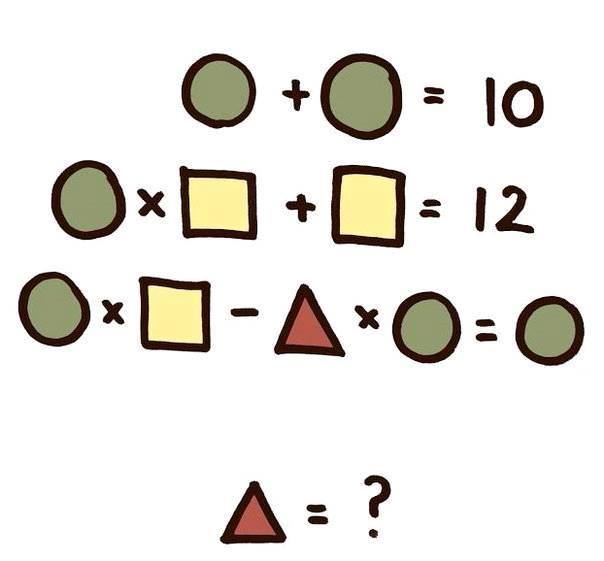
\includegraphics[scale=0.3]{SMT/equation.jpg}
\caption{System of equations}
\end{figure}

It's that easy to solve it in Z3 \ac{SMT}-solver:

\begin{lstlisting}
#!/usr/bin/python
from z3 import *

circle, square, triangle = Ints('circle square triangle')
s = Solver()
s.add(circle+circle==10)
s.add(circle*square+square==12)
s.add(circle*square-triangle*circle==circle)
print s.check()
print s.model()
\end{lstlisting}

\begin{lstlisting}
sat
[triangle = 1, square = 2, circle = 5]
\end{lstlisting}

\subsection{Finding modular inverse}

And now one useful equation.

It's possible to replace division operation (slow) by multiplication (faster).
Read \href{http://beginners.re/15-Nov-2015/Reverse_Engineering_for_Beginners-en.pdf#page=490&zoom=auto,-107,806}{here} or \href{http://yurichev.com/blog/modulo/}{here} about it.

In shortest possible terms, here is how it works.

If you need to divide integer by 13, this is the same as multiplication it by $\frac{1}{13}$.
But you operate on integer numbers (\ac{CPU} registers) and can't use ratios.

Given the fact that the division by $2^n$ on \ac{CPU} occurring at lightning speed, we can reformulate the problem as:

\begin{center}
{\Large $\frac{x}{13} = x \cdot \frac{1}{13} = x \cdot \frac{M}{2^n} = \frac{x \cdot M}{2^n}$ }
\end{center}

... where $M$ is \textit{magic coefficient} and $n$ is usually started at register width in bits (32 or 64).

But how to find \textit{magic coefficient}?
This equation is to be solved:

\begin{center}
{\Large $17 \cdot x = 1+k \cdot 2^{64}$ }
\end{center}

This is a little overkill to use SMT-solver to solve this equation
\footnote{\url{https://en.wikipedia.org/wiki/Extended_Euclidean_algorithm} is usually used:
\url{http://rosettacode.org/wiki/Modular\_inverse}}, but still possible:

\begin{lstlisting}
(declare-const x Int)
(declare-const k Int)
(assert (> x 0))
(assert (> k 0))
(assert (=
		(* 17 x)
		(+ 1 (* k (^ 2 64)))
	)
)
(check-sat)
(get-model)
\end{lstlisting}

Important note: we use \textit{Int} sort here, because this is Diophantine equation (i.e., only integer solutions are allowed).
Resulting code will run on integer \ac{CPU} registers, after all.

Z3 gave this:

% FIXME:
\begin{lstlisting}
\$ z3 -smt2 1.smt
sat
(model
  (define-fun k () Int
    16)
  (define-fun x () Int
    17361641481138401521)
)
\end{lstlisting}

Let's check:

% FIXME:
\begin{lstlisting}
#include <stdint.h>
#include <stdio.h>

uint64_t div_by_17 (uint64_t x)
{
	__int128 result = (__int128)x * (__int128)17361641481138401521UL;
	return result >> 64 >> 4;
};

int main()
{
	printf ("%lld\n", 123456789/17);
	printf ("%lld\n", div_by_17(123456789));
};
\end{lstlisting}

... and it works.

GCC doesn't use 128-bit registers, it just exploit the fact that x86 multiplication instruction produces 128-bit result, lower 64-bit part in RAX register,
and higher 64-bit part in RDX register.
In standard C/C++ it's not possible to access higher part, so this hack is helpful.

This is what optimizing GCC 4.8.4 generates:

\begin{lstlisting}
div_by_17:
        movabs  rax, -1085102592571150095
        mul     rdi
        mov     rax, rdx
        sar     rax, 4
        ret
\end{lstlisting}

Z3 may give ``unsat'' (for XXX) % 10?
if there is no integer solution for the equation (but real solution may exist).



\subsection{Connection between \ac{SAT} and \ac{SMT} solvers}

Early \ac{SMT}-solvers were frontends to \ac{SAT} solvers, i.e., they translating input SMT expressions into \ac{CNF} and feed SAT-solver with it.
Conversion process is sometimes called ``bit blasting''.
Some \ac{SMT}-solvers still works in that way: STP uses MiniSAT or CryptoMiniSAT as backend SAT-solver.
Some other \ac{SMT}-solvers are more advanced (like Z3), so they use something even more complex.

% subsections
\subsection{Zebra puzzle (AKA Einstein puzzle)} % FIXME \ac

Zebra puzzle is a popular puzzle, defined as follows:

% FIXME remove paragraph at first line
\begin{framed}
\begin{quotation}
1.There are five houses.\\
2.The Englishman lives in the red house.\\
3.The Spaniard owns the dog.\\
4.Coffee is drunk in the green house.\\
5.The Ukrainian drinks tea.\\
6.The green house is immediately to the right of the ivory house.\\
7.The Old Gold smoker owns snails.\\
8.Kools are smoked in the yellow house.\\
9.Milk is drunk in the middle house.\\
10.The Norwegian lives in the first house.\\
11.The man who smokes Chesterfields lives in the house next to the man with the fox.\\
12.Kools are smoked in the house next to the house where the horse is kept.\\
13.The Lucky Strike smoker drinks orange juice.\\
14.The Japanese smokes Parliaments.\\
15.The Norwegian lives next to the blue house.\\
\\
Now, who drinks water? Who owns the zebra?\\
\\
In the interest of clarity, it must be added that each of the five houses is painted a different color, and their inhabitants are of different national extractions, own different pets, drink different beverages and smoke different brands of American cigarets [sic]. One other thing: in statement 6, right means your right.
\end{quotation}
\end{framed}
( \url{https://en.wikipedia.org/wiki/Zebra_Puzzle} ) \\
\\
It's a very good example of constraint satisfaction problem (CSP). % FIXME \ac

We would encode each entity as integer variable, representing number of house.

Then, to define that Englishman lives in red house, we will define this constraint: \texttt{Englishman == Red}, meaning that number of a house where Englishmen resides and where tea is drunk is the same.

To define that Norwegian lives next to the blue house, we don't realy know, if it is at left side of blue house or at right side, but we know that house numbers are different by just 1.
So we will define this constraint: \texttt{Norwegian==Blue-1 OR Norwegian==Blue+1}.

We will also need to limit all house numbers, so they will be in range of 1..5.

We will also use \texttt{Distinct} to show that all various entities of the same type are all has different house numbers.

\lstinputlisting{SMT/zebra.py}

When we run it, we got correct result:

\begin{lstlisting}
sat
[Snails = 3,
 Blue = 2,
 Ivory = 4,
 OrangeJuice = 4,
 Parliament = 5,
 Yellow = 1,
 Fox = 1,
 Zebra = 5,
 Horse = 2,
 Dog = 4,
 Tea = 2,
 Water = 1,
 Chesterfield = 2,
 Red = 3,
 Japanese = 5,
 LuckyStrike = 4,
 Norwegian = 1,
 Milk = 3,
 Kools = 1,
 OldGold = 3,
 Ukrainian = 2,
 Coffee = 5,
 Green = 5,
 Spaniard = 4,
 Englishman = 3]
 \end{lstlisting}


\subsection{Sudoku puzzle}
\label{sudoku_SMT}

Sudoku puzzle is a 9*9 grid with some cells filled, some are left to be found:

% copypasted from http://www.texample.net/tikz/examples/sudoku/
\newcounter{row}
\newcounter{col}

\newcommand\setrow[9]{
  \setcounter{col}{1}
  \foreach \n in {#1, #2, #3, #4, #5, #6, #7, #8, #9} {
    \edef\x{\value{col} - 0.5}
    \edef\y{9.5 - \value{row}}
    \node[anchor=center] at (\x, \y) {\n};
    \stepcounter{col}
  }
  \stepcounter{row}
}

\begin{center}
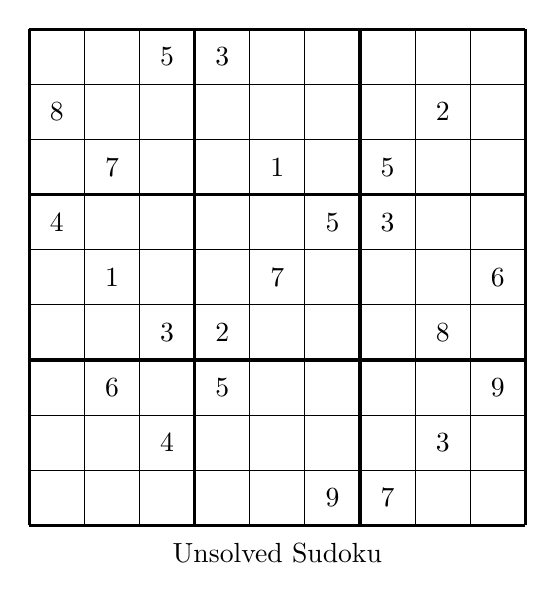
\begin{tikzpicture}[scale=.7]
  \begin{scope}
    \draw (0, 0) grid (9, 9);
    \draw[very thick, scale=3] (0, 0) grid (3, 3);

    \setcounter{row}{1}
    \setrow { }{ }{5}  {3}{ }{ }  { }{ }{ }
    \setrow {8}{ }{ }  { }{ }{ }  { }{2}{ }
    \setrow { }{7}{ }  { }{1}{ }  {5}{ }{ }

    \setrow {4}{ }{ }  { }{ }{5}  {3}{ }{ }
    \setrow { }{1}{ }  { }{7}{ }  { }{ }{6}
    \setrow { }{ }{3}  {2}{ }{ }  { }{8}{ }

    \setrow { }{6}{ }  {5}{ }{ }  { }{ }{9}
    \setrow { }{ }{4}  { }{ }{ }  { }{3}{ }
    \setrow { }{ }{ }  { }{ }{9}  {7}{ }{ }

    \node[anchor=center] at (4.5, -0.5) {Unsolved Sudoku};
  \end{scope}
\end{tikzpicture}
\end{center}

Numbers of each row must be unique, i.e., must contain all 9 numbers in range of 1..9 without repetition.
Same story for each column and also for each 3*3 square.

This puzzle is good candidate to try \ac{SMT} solver on, because it's essentially an unsolved system of equations.

\subsubsection{The first idea}

The only thing we must solve is that how to determine in one expression, if the input 9 variables has all 9 unique numbers?
They are not ordered or sorted, after all.

From the school-level mathematics, we can devise this idea:

\begin{equation}
\underbrace{10^{i_1} + 10^{i_2} + \cdots + 10^{i_9}}_9 = 1111111110
\end{equation}

Take each input variable, calculate $10^i$ and sum them all.
If all input values are unique, each will be settled at its own place.
Even more than that: there will be no holes, i.e., no skipped values.
So, in case of Sudoku, 1111111110 number will be final result, indicating that all 9 input variables are unique, in range of 1..9.

Exponentiation is heavy operation, can we use binary operations? Yes, just replace 10 with 2:

\begin{equation}
\underbrace{2^{i_1} + 2^{i_2} + \cdots + 2^{i_9}}_9 = 1111111110_2
\end{equation}

The effect is just the same, but the final value is in base 2 instead of 10.

Now a working example:

\lstinputlisting{SMT/sudoku_plus.py}
( \url{https://github.com/dennis714/SAT_SMT_article/blob/master/SMT/sudoku_plus.py} )

\begin{lstlisting}
% time python sudoku_plus.py
1 4 5 3 2 7 6 9 8
8 3 9 6 5 4 1 2 7
6 7 2 9 1 8 5 4 3
4 9 6 1 8 5 3 7 2
2 1 8 4 7 3 9 5 6
7 5 3 2 9 6 4 8 1
3 6 7 5 4 2 8 1 9
9 8 4 7 6 1 2 3 5
5 2 1 8 3 9 7 6 4

real    0m11.717s
user    0m10.896s
sys     0m0.068s
\end{lstlisting}

Even more, we can replace summing operation to logical OR:

\begin{equation}
\underbrace{2^{i_1} \vee 2^{i_2} \vee \cdots \vee 2^{i_9}}_9 = 1111111110_2
\end{equation}

% FIXME: только часть исходника
\lstinputlisting{SMT/sudoku_or.py}
( \url{https://github.com/dennis714/SAT_SMT_article/blob/master/SMT/sudoku_or.py} )

Now it works much faster. Z3 handles OR operation over bit vectors better than addition?

\begin{lstlisting}
% time python sudoku_or.py
1 4 5 3 2 7 6 9 8
8 3 9 6 5 4 1 2 7
6 7 2 9 1 8 5 4 3
4 9 6 1 8 5 3 7 2
2 1 8 4 7 3 9 5 6
7 5 3 2 9 6 4 8 1
3 6 7 5 4 2 8 1 9
9 8 4 7 6 1 2 3 5
5 2 1 8 3 9 7 6 4

real    0m1.429s
user    0m1.393s
sys     0m0.036s
\end{lstlisting}

The puzzle I used as example is dubbed as one of the hardest known
\footnote{\url{http://www.mirror.co.uk/news/weird-news/worlds-hardest-sudoku-can-you-242294}} (well, for humans).
It took \~1.4 seconds on my Intel Core i3-3110M 2.4GHz notebook to solve it.

\subsubsection{The second idea}

My first approach is far from effective, I did what first came to my mind and worked.
Another approach is to use \TT{distinct} command from SMTLIB, which tells Z3 that some variables (of unspecific number) must be distinct (or unique).
This command is also available in Z3 Python interface.

I've rewritten my first Sudoku solver, now it operates over \textit{Int} \textit{sort}, it has \TT{distinct} commands instead of bit operations,
and now also other constaint added: each cell value must be in 1..9 range, because, otherwise, Z3 will offer (although correct) solution with too big
and/or negative numbers.

% FIXME: только часть исходника
\lstinputlisting{SMT/sudoku2.py}
( \url{https://github.com/dennis714/SAT_SMT_article/blob/master/SMT/sudoku2.py} )

\begin{lstlisting}
% time python sudoku2.py
1 4 5 3 2 7 6 9 8
8 3 9 6 5 4 1 2 7
6 7 2 9 1 8 5 4 3
4 9 6 1 8 5 3 7 2
2 1 8 4 7 3 9 5 6
7 5 3 2 9 6 4 8 1
3 6 7 5 4 2 8 1 9
9 8 4 7 6 1 2 3 5
5 2 1 8 3 9 7 6 4

real    0m0.382s
user    0m0.346s
sys     0m0.036s
\end{lstlisting}

That's much faster.

\subsubsection{Conclusion}

The awesomeness of \ac{SMT}-solvers is that our Sudoku solver has nothing else, we have just defined relationships between variables (cells).

\subsubsection{Homework}

As it seems, true Sudoku puzzle is the one which has only one solution.
The piece of code I've included in this article shows only the first one.
Using the method described earlier (\ref{SMTEnumerate}, also called ``model counting''), 
try to find more solutions, or prove that the solution you have just found is the only one possible.

\subsubsection{Further reading}

\url{http://www.norvig.com/sudoku.html}

\subsubsection{Sudoku as a \ac{SAT} problem}

It's also possible to represend Sudoku puzzle as a huge \ac{CNF} equation and use \ac{SAT}-solver to find solution, but it's just trickier.

Some articles about it:
\textit{Building a Sudoku Solver with SAT}\footnote{\url{http://ocw.mit.edu/courses/electrical-engineering-and-computer-science/6-005-elements-of-software-construction-fall-2011/assignments/MIT6_005F11_ps4.pdf}},
Tjark Weber, \textit{A SAT-based Sudoku Solver}\footnote{\url{https://www.lri.fr/~conchon/mpri/weber.pdf}},
Ines Lynce, Joel Ouaknine, \textit{Sudoku as a SAT Problem}\footnote{\url{http://sat.inesc-id.pt/~ines/publications/aimath06.pdf}},
Gihwon Kwon, Himanshu Jain, \textit{Optimized CNF Encoding for Sudoku Puzzles}\footnote{\url{http://www.cs.cmu.edu/~hjain/papers/sudoku-as-SAT.pdf}}.

\ac{SMT}-solver can also use \ac{SAT}-solver in its core, so it does all mundane translating work.
As a ``compiler'', it may not do this in the most efficient way, though.


\subsection{Solving Problem Euler 31 - ``Coin sums''}

(This post was first published in my blog\footnote{\url{http://dennisyurichev.blogspot.de/2013/05/in-england-currency-is-made-up-of-pound.html}} at 10-May-2013).

\begin{framed}
\begin{quotation}
In England the currency is made up of pound, £, and pence, p, and there are eight coins in general circulation:

1p, 2p, 5p, 10p, 20p, 50p, £1 (100p) and £2 (200p).
It is possible to make £2 in the following way:

1£1 + 150p + 220p + 15p + 12p + 31p
How many different ways can £2 be made using any number of coins?
\end{quotation}
\end{framed}
( \href{http://projecteuler.net/problem=31}{Problem Euler 31 - Coin sums} )

\label{SMTEnumerate}
Using Z3 \ac{SMT} solver for solving this is overkill, and also slow, but nevertheless, it works, showing all possible solutions as well.
The piece of code for blocking already found solution and search for next, and thus, counting all solutions, was taken from Stack Overflow answer
\footnote{\url{http://stackoverflow.com/questions/11867611/z3py-checking-all-solutions-for-equation}, 
another question: \url{http://stackoverflow.com/questions/13395391/z3-finding-all-satisfying-models}}.
This is also called ``model counting''.
Constraints like ``a>=0'' must be present, because Z3 solver will search for solutions with negative numbers.

\begin{lstlisting}
#!/usr/bin/python

from z3 import *

a,b,c,d,e,f,g,h = Ints('a b c d e f g h')
s = Solver()
s.add(1*a + 2*b + 5*c + 10*d + 20*e + 50*f + 100*g + 200*h == 200, 
   a>=0, b>=0, c>=0, d>=0, e>=0, f>=0, g>=0, h>=0)
result=[]

while True:
    if s.check() == sat:
        m = s.model()
        print m
        result.append(m)
        # Create a new constraint the blocks the current model
        block = []
        for d in m:
            # d is a declaration
            if d.arity() > 0:
                raise Z3Exception("uninterpreted functions are not suppported")
            # create a constant from declaration
            c=d()
            #print c, m[d]
            if is_array(c) or c.sort().kind() == Z3_UNINTERPRETED_SORT:
                raise Z3Exception("arrays and uninterpreted sorts are not supported")
            block.append(c != m[d])
        #print "new constraint:",block
        s.add(Or(block))
    else:
        print len(result)
        break
\end{lstlisting}

Works very slow, and this is what it produces:

\begin{lstlisting}
[h = 0, g = 0, f = 0, e = 0, d = 0, c = 0, b = 0, a = 200]
[f = 1, b = 5, a = 0, d = 1, g = 1, h = 0, c = 2, e = 1]
[f = 0, b = 1, a = 153, d = 0, g = 0, h = 0, c = 1, e = 2]
...
[f = 0, b = 31, a = 33, d = 2, g = 0, h = 0, c = 17, e = 0]
[f = 0, b = 30, a = 35, d = 2, g = 0, h = 0, c = 17, e = 0]
[f = 0, b = 5, a = 50, d = 2, g = 0, h = 0, c = 24, e = 0]
\end{lstlisting}

73682 results in total.

\subsection{Using Z3 theorem prover to prove equivalence of some weird alternative to XOR operation}

(The article was first published in my blog at April 2015: \url{http://blog.yurichev.com/node/86}).

There is a "A Hacker's Assistant" program\footnote{\url{http://www.hackersdelight.org/}} (\textit{Aha!}) written by Henry Warren,
who is also the author of the great "Hacker's Delight" book.

The \textit{Aha!} program is essentially \textit{superoptimizer}\footnote{\url{http://en.wikipedia.org/wiki/Superoptimization}},
which blindly brute-force a list of some generic RISC CPU instructions to achieve shortest possible (and jumpless or branch-free) 
CPU code sequence for desired operation.
One of the impressive examples of its work is finding of Dietz's formula\footnote{\url{http://aggregate.org/MAGIC/\#Average\%20of\%20Integers}},
which is the code of computing average number of two numbers without overflow (which is important if you want to find average number of numbers like 0xFFFFFF00 and so on, using 32-bit registers).
Taking this in input:

\begin{lstlisting}
int userfun(int x, int y) {     // To find Dietz's formula for
                                // the floor-average of two
                                // unsigned integers.
   return ((unsigned long long)x + (unsigned long long)y) >> 1;
}
\end{lstlisting}

... the \textit{Aha!} gives this:

\begin{lstlisting}
Found a 4-operation program:
   and   r1,ry,rx
   xor   r2,ry,rx
   shrs  r3,r2,1
   add   r4,r3,r1
   Expr: (((y ^ x) >>s 1) + (y & x))
\end{lstlisting}

And it works correctly.

\textit{Aha!} can also find jumpless version of abs() function easily.

Compiler developers use superoptimization to find shortest possible (and/or jumpless) code, but I tried to do otherwise -- to find longest code for some basic operation.
I tried \textit{Aha!} to find equivalent of basic XOR operation without usage of the actual XOR instruction, and the most bizarre example \textit{Aha!} gave is:

\begin{lstlisting}
Found a 4-operation program:
   add   r1,ry,rx
   and   r2,ry,rx
   mul   r3,r2,-2
   add   r4,r3,r1
   Expr: (((y & x)*-2) + (y + x))
\end{lstlisting}

And it's hard to say, why/where we can use it, maybe for obfuscation, I'm not sure.
I would call this \textit{suboptimization} (as opposed to \textit{superoptimization}). Or maybe \textit{superdeoptimization}.

But my another question was also, is it possible to prove that this is correct formula at all?
The \textit{Aha!} checking some intput/output values against XOR operation, but of course, not all the possible values.
It is 32-bit code, so it may take very long time to try all possible 32-bit inputs to test it.

We can try Z3 theorem prover for the job. It's called ``prover'', after all.

So I wrote this:

\begin{lstlisting}
#!/usr/bin/python
from z3 import *

x = BitVec('x', 32)
y = BitVec('y', 32)
output = BitVec('output', 32)
s = Solver()
s.add(x^y==output)
s.add(((y & x)*0xFFFFFFFE) + (y + x)!=output)
print s.check()
\end{lstlisting}

In plain English language, this means "are there any case for x and y where $x \oplus y$ doesn't equals to $((y \& x)*-2) + (y + x)$?"
... and Z3 prints "unsat", meaning, it can't find any counterexample to the equation.
So this \textit{Aha!} output is proved to be working just like XOR operation.

Oh, I also tried to extend the formula to 64-bit:

\begin{lstlisting}
#!/usr/bin/python
from z3 import *

x = BitVec('x', 64)
y = BitVec('y', 64)
output = BitVec('output', 64)
s = Solver()
s.add(x^y==output)
s.add(((y & x)*0xFFFFFFFE) + (y + x)!=output)
print s.check()
\end{lstlisting}

Nope, now it says "sat", meaning, Z3 found at least one counterexample.
Oops, it's because I forgot to extend -2 number to 64-bit value:

\begin{lstlisting}
#!/usr/bin/python
from z3 import *

x = BitVec('x', 64)
y = BitVec('y', 64)
output = BitVec('output', 64)
s = Solver()
s.add(x^y==output)
s.add(((y & x)*0xFFFFFFFFFFFFFFFE) + (y + x)!=output)
print s.check()
\end{lstlisting}

Now it says "unsat", so the formula given by \textit{Aha!} works for 64-bit code as well.

\subsubsection{In SMT-LIB form}

Now we can rephrase our equation to more suitable form: $(x + y - ((x \& y)<<1))$.
It also works well is Z3:

\begin{lstlisting}
#!/usr/bin/python
from z3 import *

x = BitVec('x', 64)
y = BitVec('y', 64)
output = BitVec('output', 64)
s = Solver()
s.add(x^y==output)
s.add((x + y - ((x & y)<<1)) != output)
print s.check()
\end{lstlisting}

Here is how to define it in SMT-LIB way:

\begin{lstlisting}
(declare-const x (_ BitVec 64))
(declare-const y (_ BitVec 64))
(assert (not (=(bvsub (bvadd x y) (bvshl (bvand x y) (_ bv1 64))) (bvxor x y))))
(check-sat)
\end{lstlisting}

\subsubsection{Using universal quantifier}

Z3 has universal quantifier \TT{forall}, which defines a constraint, where all possible values for the equation must be true.
So we can rewrite our SMT example as:

\begin{lstlisting}
(declare-const x (_ BitVec 64))
(declare-const y (_ BitVec 64))
(forall (=(bvsub (bvadd x y) (bvshl (bvand x y) (_ bv1 64))) (bvxor x y)))
(check-sat)
\end{lstlisting}

It returns \TT{sat}, meaning, the equation is correct for all \TT{x} and \TT{y} values.

Mathematically speaking: $\forall n\!\in\!\mathbb{N}\; (x \oplus y = (x + y - ((x \& y)<<1)))$
\footnote{
$\forall$ means \textit{equation must be true for all possible values}, which are choosen from natural numbers ($\mathbb{N}$).}

\subsubsection{How the equation works}

First of all, binary addition can be viewed as binary XORing with carrying (\ref{adder}).
Here is an example: let's add 2 (10b) and 2 (10b).
XORing these two values resulting 0, but there is a carry generated during addition of two second bits.
That carry bit is propagated further and settles at the place of the 3rd bit: 100b.
4 (100b) is hence a final result of addition.

If the carry bits are not generated during addition, the addition operation is merely XORing.
For example, let's add 1 (1b) and 2 (10b). $1 + 2$ equals to 3, but $1 \oplus 2$ is also 3.

If the addition is XORing plus carry generation and application, we should eliminate effect of carrying somehow here.
The first part of the equation ($x + y$) is addition, the second ($(x \& y)<<1$) is just calculation of every carry bit which was used during addition.
Subtracting removes carry bits from the result of addition, so the only XOR effect is left then.

It's hard to say how Z3 proves this: maybe it just simplifies the equation down to single XOR using simple boolean algebra rewriting rules?

   % \\
\subsection{Dietz's formula}

Now something practical and useful.

One of the impressive examples of \textit{Aha!} work is finding of Dietz's formula\footnote{\url{http://aggregate.org/MAGIC/\#Average\%20of\%20Integers}},
which is the code of computing average number of two numbers without overflow (which is important if you want to find average number of numbers like 0xFFFFFF00 and so on, using 32-bit registers).
Taking this in input:

\begin{lstlisting}
int userfun(int x, int y) {     // To find Dietz's formula for
                                // the floor-average of two
                                // unsigned integers.
   return ((unsigned long long)x + (unsigned long long)y) >> 1;
}
\end{lstlisting}

... the \textit{Aha!} gives this:

\begin{lstlisting}
Found a 4-operation program:
   and   r1,ry,rx
   xor   r2,ry,rx
   shrs  r3,r2,1
   add   r4,r3,r1
   Expr: (((y ^ x) >>s 1) + (y & x))
\end{lstlisting}

And it works correctly\footnote{For those who interesting how it works, its mechanics is closely related to the weird XOR alternative we just saw.
That's why I placed these two pieces of text one after another.}.
But how to prove it?

We will place Dietz's formula on the left side of equation and $x+y/2$ (or $x+y>>1$) on the right side:

\begin{center}
$\forall n \in 0..2^{64}-1 . (x\&y) + (x \oplus y)>>1 = x+y>>1$
\end{center}

One important thing is that we can't operate on 64-bit values on right side, because result will overflow.
So we will zero extend inputs on right side by 1 bit (in other words, we will just 1 zero bit before each variable).
The result of Dietz's formula will also be extended by 1 bit.
Hence, both sides of the equation will have a width of 64 bits:

\begin{lstlisting}
(declare-const x (_ BitVec 64))
(declare-const y (_ BitVec 64))
(assert 
	(forall ((x (_ BitVec 64)) (y (_ BitVec 64)))
		(=
			((_ zero_extend 1)
				(bvadd
					(bvand x y)
					(bvlshr (bvxor x y) (_ bv1 64))
				)
			)
			(bvlshr
				(bvadd ((_ zero_extend 1) x) ((_ zero_extend 1) y))
				(_ bv1 65)
			)
		)
	)
)
(check-sat)
\end{lstlisting}

Z3 says ``sat''.\\
\\
65 bits are enough, because the result of addition of two biggest 64-bit values has width of 65 bits: \\
\TT{0xFF...FF + 0xFF...FF = 0x1FF...FE}.\\
\\
As in previous example about XOR equivalent, \TT{(not (= ... ))} and \TT{exists} can also be used here instead of \TT{forall}.

 % //
\subsection{Cracking \ac{LCG} with Z3 \ac{SMT} solver}

This part is first appeared in my blog in June 2015 at \url{http://yurichev.com/blog/modulo/}.

There are well-known weaknesses of LCG (
\href{http://en.wikipedia.org/wiki/Linear_congruential_generator#Advantages_and_disadvantages_of_LCGs}{1},
\href{http://www.reteam.org/papers/e59.pdf}{2},
\href{http://stackoverflow.com/questions/8569113/why-1103515245-is-used-in-rand/8574774#8574774}{3}
), but let's see, if it would be possible to crack it straightforwardly, without any special knowledge.
We would define all relations between LCG states in term of Z3 \ac{SMT} solver.
(I first made attempt to do it using \href{https://reference.wolfram.com/language/ref/FindInstance.html}{FindInstance} in Wolfram Mathematica, but failed, perhaps, made a mistake somewhere).
Here is a test progam:

\begin{lstlisting}
#include <stdlib.h>
#include <stdio.h>
#include <time.h>

int main()
{
	int i;

	srand(time(NULL));

	for (i=0; i<10; i++)
		printf ("%d\n", rand()%100);
};
\end{lstlisting}

It is intended to print 10 pseudorandom numbers in 0..99 range.
So it does:

\begin{lstlisting}
37
29
74
95
98
40
23
58
61
17
\end{lstlisting}

Let's say we are observing only 8 of these numbers (from 29 to 61) and we need to predict next one (17) and/or previous one (37).

The program is compiled using MSVC 2013 (I choose it because its LCG is simpler than that in Glib):

\begin{lstlisting}
.text:0040112E rand            proc near
.text:0040112E                 call    __getptd
.text:00401133                 imul    ecx, [eax+0x14], 214013
.text:0040113A                 add     ecx, 2531011
.text:00401140                 mov     [eax+14h], ecx
.text:00401143                 shr     ecx, 16
.text:00401146                 and     ecx, 7FFFh
.text:0040114C                 mov     eax, ecx
.text:0040114E                 retn
.text:0040114E rand            endp
\end{lstlisting}

This is very simple LCG, but the result is not clipped state, but it's rather shifted by 16 bits.
Let's define LCG in Z3:

\begin{lstlisting}
#!/usr/bin/python
from z3 import *

output_prev = BitVec('output_prev', 32)
state1 = BitVec('state1', 32)
state2 = BitVec('state2', 32)
state3 = BitVec('state3', 32)
state4 = BitVec('state4', 32)
state5 = BitVec('state5', 32)
state6 = BitVec('state6', 32)
state7 = BitVec('state7', 32)
state8 = BitVec('state8', 32)
state9 = BitVec('state9', 32)
state10 = BitVec('state10', 32)
output_next = BitVec('output_next', 32)

s = Solver()

s.add(state2 == state1*214013+2531011)
s.add(state3 == state2*214013+2531011)
s.add(state4 == state3*214013+2531011)
s.add(state5 == state4*214013+2531011)
s.add(state6 == state5*214013+2531011)
s.add(state7 == state6*214013+2531011)
s.add(state8 == state7*214013+2531011)
s.add(state9 == state8*214013+2531011)
s.add(state10 == state9*214013+2531011)

s.add(output_prev==URem((state1>>16)&0x7FFF,100))
s.add(URem((state2>>16)&0x7FFF,100)==29)
s.add(URem((state3>>16)&0x7FFF,100)==74)
s.add(URem((state4>>16)&0x7FFF,100)==95)
s.add(URem((state5>>16)&0x7FFF,100)==98)
s.add(URem((state6>>16)&0x7FFF,100)==40)
s.add(URem((state7>>16)&0x7FFF,100)==23)
s.add(URem((state8>>16)&0x7FFF,100)==58)
s.add(URem((state9>>16)&0x7FFF,100)==61)
s.add(output_next==URem((state10>>16)&0x7FFF,100))

print(s.check())
print(s.model())
\end{lstlisting}

URem states for \textit{unsigned remainder}.
It works for some time and gave us correct result!

\begin{lstlisting}
sat
[state3 = 2276903645,
 state4 = 1467740716,
 state5 = 3163191359,
 state7 = 4108542129,
 state8 = 2839445680,
 state2 = 998088354,
 state6 = 4214551046,
 state1 = 1791599627,
 state9 = 548002995,
 output_next = 17,
 output_prev = 37,
 state10 = 1390515370]
\end{lstlisting}

% FIXME tilde
I added ~10 states to be sure result will be correct. It may be not if you supply lesser amount of PRNG numbers.

That is the reason why LCG is not suitable for any security-related task.
This is why \href{https://en.wikipedia.org/wiki/Cryptographically_secure_pseudorandom_number_generator}{cryptographically secure pseudorandom number generators} exist: they are designed to be protected against such simple attack.
Well, at least if \href{https://en.wikipedia.org/wiki/Dual_EC_DRBG}{NSA is not involved}.

As far, as I can understand, \href{http://en.wikipedia.org/wiki/Security_token}{security tokens} like \href{http://en.wikipedia.org/wiki/RSA_SecurID}{RSA SecurID} can be viewed just as \ac{CPRNG} with a secret seed.
It shows new pseudorandom number each minute, and the server can predict it, because it knows the seed.
Imagine if such token would implement LCG -- it would be much easier to break!


\subsection{Solving pipe puzzle using Z3 SMT-solver}

``Pipe puzzle'' is a popular puzzle (just google ``pipe puzzle'' and look at images).

This is how shuffled puzzle looks like:

\begin{figure}[H]
\label{fig:pipe_shuffled}
\centering
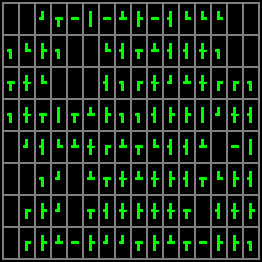
\includegraphics[scale=0.75]{SMT/pipe/shuffled.png}
\caption{Shuffled puzzle}
\end{figure}

\dots and solved:

\begin{figure}[H]
\label{fig:pipe_solved}
\centering
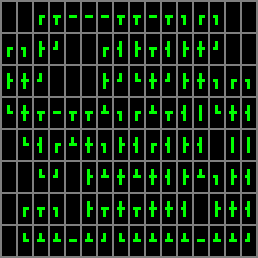
\includegraphics[scale=0.75]{SMT/pipe/solved.png}
\caption{Solved puzzle}
\end{figure}

Let's try to find a way to solve it.

\subsubsection{Generation}

First, we need to generate it.
Here is my quick idea on it.
Take 8*16 array of cells.
Each cell may contain some kind of block.
There are joints between cells:

\pgfmathsetmacro\Width{16}
\pgfmathsetmacro\Height{8}
%\pgfmathsetmacro\Width{10}
%\pgfmathsetmacro\Height{5}
\pgfmathtruncatemacro\WidthMinusI{\Width - 1}
\pgfmathtruncatemacro\WidthMinusII{\Width - 2}
\pgfmathtruncatemacro\HeightMinusI{\Height - 1}
\pgfmathtruncatemacro\HeightMinusII{\Height - 2}
\pgfmathtruncatemacro\HeightPlusII{\Height + 2}
\pgfmathsetmacro\HeightPlusIi{\Height + 1.5}

% see also: http://www.texample.net/tikz/examples/euclid-algorithm/
\begin{center}
\begin{tikzpicture}[set style={{help lines}+=[dashed]},scale=0.7]

	\draw[style=help lines] (0,0) grid +(\Width,\Height);

	\foreach \c in {0,...,\WidthMinusI}
	{
		\foreach \r in {0,...,\HeightMinusII}
			\draw   [red,very thick,-] (\c+0.5,\r+0.75) -- (\c+0.5,\r+1.25);
		%\node[rotate=90] at (\c+0.5,\HeightPlusII) {\Large vjoints[\dots, \c] \normalsize};
		\node[rotate=90] at (\c+0.5,\HeightPlusII) {vjoints[\dots, \c]};
	}

	\foreach \r in {0,...,\HeightMinusI}
	{
		\foreach \c in {0,...,\WidthMinusII}
			\draw   [blue,very thick,-] (\c+0.75,\r+0.5) -- (\c+1.25,\r+0.5);
		\pgfmathtruncatemacro\hjointslabel{\HeightMinusI - \r}
		%\node at (-1.5,\r+0.5) {\large hjoints[\hjointslabel, \dots] \normalsize};
		\node at (-1.5,\r+0.5) {hjoints[\hjointslabel, \dots]};
	}

\end{tikzpicture}
\end{center}



Blue lines are horizontal joints, red lines are vertical joints.
We just set each joint to 0/false (absent) or 1/true (present), randomly.

Once set, it's now easy to find type for each cell.
There are:

\newcommand{\HeaderColor}{\cellcolor{blue!25}}
\begin{center}
\begin{longtable}{ | l | l | l | l | }
\hline
\HeaderColor joints & \HeaderColor our internal name & \HeaderColor angle & \HeaderColor symbol \\
\hline
0	&type 0		&	0$^{\circ}$	& (space)	\\
2	&type 2a	&	0$^{\circ}$	& \pmboxdrawuni{2503} \\ % ┃
2	&type 2a	&	90$^{\circ}$	& \pmboxdrawuni{2501} \\ % ━
2	&type 2b	&	0$^{\circ}$	& \pmboxdrawuni{250F} \\ % ┏
2	&type 2b	&	90$^{\circ}$	& \pmboxdrawuni{2513} \\ % ┓
2	&type 2b	&	180$^{\circ}$	& \pmboxdrawuni{251B} \\ % ┛
2	&type 2b	&	270$^{\circ}$	& \pmboxdrawuni{2517} \\ % ┗
3	&type 3		&	0$^{\circ}$	& \pmboxdrawuni{2523} \\ % ┣
3 	&type 3		&	90$^{\circ}$	& \pmboxdrawuni{2533} \\ % ┳
3	&type 3		&	180$^{\circ}$	& \pmboxdrawuni{252B} \\ % ┫
3	&type 3		&	270$^{\circ}$	& \pmboxdrawuni{253B} \\ % ┻
4	&type 4		&	0$^{\circ}$	& \pmboxdrawuni{254B} \\ % ╋
\hline
\end{longtable}
\end{center}

Dangling joints are possible at the first stage (i.e., cell with only one joint), but they are removed recursively,
these cells are transforming into empty cells.
Hence, at the end, all cells has at least two joints, and the whole plumbing system has no connections with outer
world---I hope this would make things clearer.

The C source code of generator is here: \url{https://github.com/dennis714/SAT_SMT_article/tree/master/SMT/pipe/generator}.
All horizontal joints are in global array \textit{hjoints[]} and vertical in \textit{vjoints[]}.

The C program generates ANSI-colored output like it has been showed above (\ref{fig:pipe_shuffled}, \ref{fig:pipe_solved}) plus
an array of types, with no angle information about each cell:

\begin{lstlisting}[label=init_cells]
[
["0", "0", "2b", "3", "2a", "2a", "2a", "3", "3", "2a", "3", "2b", "2b", "2b", "0", "0"],
["2b", "2b", "3", "2b", "0", "0", "2b", "3", "3", "3", "3", "3", "4", "2b", "0", "0"],
["3", "4", "2b", "0", "0", "0", "3", "2b", "2b", "4", "2b", "3", "4", "2b", "2b", "2b"],
["2b", "4", "3", "2a", "3", "3", "3", "2b", "2b", "3", "3", "3", "2a", "2b", "4", "3"],
["0", "2b", "3", "2b", "3", "4", "2b", "3", "3", "2b", "3", "3", "3", "0", "2a", "2a"],
["0", "0", "2b", "2b", "0", "3", "3", "4", "3", "4", "3", "3", "3", "2b", "3", "3"],
["0", "2b", "3", "2b", "0", "3", "3", "4", "3", "4", "4", "3", "0", "3", "4", "3"],
["0", "2b", "3", "3", "2a", "3", "2b", "2b", "3", "3", "3", "3", "2a", "3", "3", "2b"],
]
\end{lstlisting}

\subsubsection{Solving}

First of all, we would think about 8*16 array of cells, where each has four bits:
``T'' (top),
``B'' (bottom),
``L'' (left),
``R'' (right).
Each bit represents half of joint.

% see also: http://www.texample.net/tikz/examples/euclid-algorithm/
\begin{center}
\begin{tikzpicture}[set style={{help lines}+=[dashed]},scale=0.7]

	\draw[style=help lines] (0,0) grid +(\Width,\Height);
	
	\foreach \c in {0,...,\WidthMinusI}
		%\node[rotate=90] at (\c+0.5,\HeightPlusIi) {\Large [\dots, \c] \normalsize};
		\node[rotate=90] at (\c+0.5,\HeightPlusIi) {[\dots, \c]};
	
	\foreach \r in {0,...,\HeightMinusI}
	{
		\pgfmathtruncatemacro\hlabel{\HeightMinusI - \r}
		%\node at (-1.5,\r+0.5) {\large [\hlabel, \dots] \normalsize};
		\node at (-1.5,\r+0.5) {[\hlabel, \dots]};
	
		\pgfmathsetmacro\Shift{0.325}
		\foreach \c in {0,...,\WidthMinusI}
		{
			\node at (\c+0.5,\r+0.5 + \Shift) {\footnotesize T \normalsize};
			\node at (\c+0.5,\r+0.5 - \Shift) {\footnotesize B \normalsize};
			\node at (\c+0.5 - \Shift,\r+0.5) {\footnotesize L \normalsize};
			\node at (\c+0.5 + \Shift,\r+0.5) {\footnotesize R \normalsize};
		}
	}

\end{tikzpicture}
\end{center}


Now we define arrays of each of four half-joints + angle information:

\begin{lstlisting}
HEIGHT=8
WIDTH=16

# if T/B/R/L is Bool instead of Int, Z3 solver will work faster
T=[[Bool('cell_%d_%d_top' % (r, c)) for c in range(WIDTH)] for r in range(HEIGHT)]
B=[[Bool('cell_%d_%d_bottom' % (r, c)) for c in range(WIDTH)] for r in range(HEIGHT)]
R=[[Bool('cell_%d_%d_right' % (r, c)) for c in range(WIDTH)] for r in range(HEIGHT)]
L=[[Bool('cell_%d_%d_left' % (r, c)) for c in range(WIDTH)] for r in range(HEIGHT)]
A=[[Int('cell_%d_%d_angle' % (r, c)) for c in range(WIDTH)] for r in range(HEIGHT)]
\end{lstlisting}

We know that if each half-joint is present, corresponding half-joint must be also present, and vice versa.
We define this using these constraints:

\begin{lstlisting}
# shorthand variables for True and False:
t=True
f=False

# "top" of each cell must be equal to "bottom" of the cell above
# "bottom" of each cell must be equal to "top" of the cell below
# "left" of each cell must be equal to "right" of the cell at left
# "right" of each cell must be equal to "left" of the cell at right
for r in range(HEIGHT):
    for c in range(WIDTH):
        if r!=0:
            s.add(T[r][c]==B[r-1][c])
        if r!=HEIGHT-1:
            s.add(B[r][c]==T[r+1][c])
        if c!=0:
            s.add(L[r][c]==R[r][c-1])
        if c!=WIDTH-1:
            s.add(R[r][c]==L[r][c+1])

# "left" of each cell of first column shouldn't have any connection
# so is "right" of each cell of the last column
for r in range(HEIGHT):
    s.add(L[r][0]==f)
    s.add(R[r][WIDTH-1]==f)

# "top" of each cell of the first row shouldn't have any connection
# so is "bottom" of each cell of the last row
for c in range(WIDTH):
    s.add(T[0][c]==f)
    s.add(B[HEIGHT-1][c]==f)
\end{lstlisting}

Now we'll enumerate all cells in the initial array (\ref{init_cells}).
First two cells are empty there. And the third one has type ``2b''.
This is ``\pmboxdrawuni{250F}'' % ┏
and it can be oriented in 4 possible ways.
And if it has angle 0$^{\circ}$, bottom half-joint and right one are present, others are absent.
If it has angle 90$^{\circ}$, it looks like 
``\pmboxdrawuni{2513}'', % ┓
and bottom and left half-joints are present, others are absent.

In plain English: ``if cell of this type has angle 0$^{\circ}$, these half-joints must be present \textbf{OR}
if it has angle 90$^{\circ}$, these half-joints must be present, \textbf{OR}, etc, etc.''

Likewise, we define all these rules for all types and all possible angles:

\begin{lstlisting}
for r in range(HEIGHT):
    for c in range(WIDTH):
        ty=cells_type[r][c]

        if ty=="0":
            s.add(A[r][c]==f)
            s.add(T[r][c]==f, B[r][c]==f, L[r][c]==f, R[r][c]==f)

        if ty=="2a":
            s.add(Or(And(A[r][c]==0, L[r][c]==f, R[r][c]==f, T[r][c]==t, B[r][c]==t),   # §\pmboxdrawuni{2503}§
                    And(A[r][c]==90, L[r][c]==t, R[r][c]==t, T[r][c]==f, B[r][c]==f)))  # §\pmboxdrawuni{2501}§

        if ty=="2b":
            s.add(Or(And(A[r][c]==0, L[r][c]==f, R[r][c]==t, T[r][c]==f, B[r][c]==t),   # §\pmboxdrawuni{250F}§
                    And(A[r][c]==90, L[r][c]==t, R[r][c]==f, T[r][c]==f, B[r][c]==t),   # §\pmboxdrawuni{2513}§
                    And(A[r][c]==180, L[r][c]==t, R[r][c]==f, T[r][c]==t, B[r][c]==f),  # §\pmboxdrawuni{251B}§
                    And(A[r][c]==270, L[r][c]==f, R[r][c]==t, T[r][c]==t, B[r][c]==f))) # §\pmboxdrawuni{2517}§
	
        if ty=="3":
            s.add(Or(And(A[r][c]==0, L[r][c]==f, R[r][c]==t, T[r][c]==t, B[r][c]==t),   # §\pmboxdrawuni{2523}§
                    And(A[r][c]==90, L[r][c]==t, R[r][c]==t, T[r][c]==f, B[r][c]==t),   # §\pmboxdrawuni{2533}§
                    And(A[r][c]==180, L[r][c]==t, R[r][c]==f, T[r][c]==t, B[r][c]==t),  # §\pmboxdrawuni{252B}§
                    And(A[r][c]==270, L[r][c]==t, R[r][c]==t, T[r][c]==t, B[r][c]==f))) # §\pmboxdrawuni{253B}§

        if ty=="4":
            s.add(A[r][c]==0)
            s.add(T[r][c]==t, B[r][c]==t, L[r][c]==t, R[r][c]==t) # §\pmboxdrawuni{254B}§
\end{lstlisting}

Full listing is here: \url{https://github.com/dennis714/SAT_SMT_article/blob/master/SMT/pipe/solver/solve_pipe_puzzle1.py}.

It produces this result (prints angle for each cell and (pseudo)graphical representation):

\begin{figure}[H]
\centering
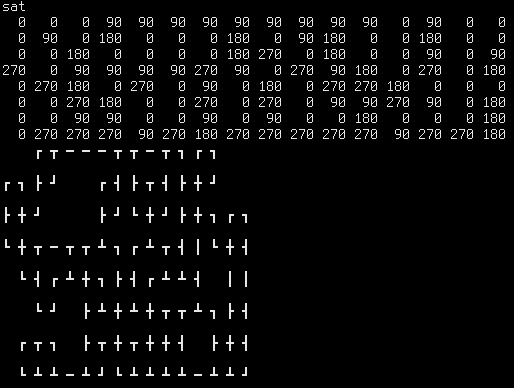
\includegraphics[scale=0.75]{SMT/pipe/solver/solver.png}
\caption{Solver script output}
\end{figure}

It worked ~4 seconds on my old and slow Intel Atom N455 1.66GHz.
Is it fast? I don't know, but again, what is really cool, we do not know about any mathematical background
of all this, we just defined cells, (half)-joints and defined relations between them.

Now the next question is, how many solutions are possible?
Using method described earlier (\ref{SMTEnumerate}), I've altered solver script
\footnote{\url{https://github.com/dennis714/SAT_SMT_article/blob/master/SMT/pipe/solver/solve_pipe_puzzle2.py}} and solver
said two solutions are possible.

Let's compare these two solutions using gvimdiff:

\begin{figure}[H]
\centering
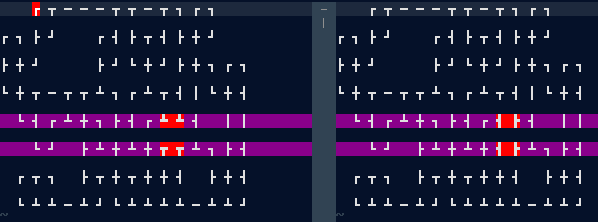
\includegraphics[scale=0.75]{SMT/pipe/solver/diff.png}
\caption{gvimdiff output (pardon my red cursor at left pane at left-bottom corner)}
\end{figure}

4 cells in the middle orientated differently.
Perhaps, other puzzles may produce different results.

P.S.
\textit{Half-joints} are defined using boolean type.
But in fact, the first version of the solver has been written using integer type for half-joints,
and 0 was used for False and 1 for True.
I did it so because I wanted to make source code tidier and narrower without using long words like ``False'' and ``True''.
And it worked, but slower. Perhaps, Z3 handles boolean data types faster? Better?
Anyway, I writing this to note that integer type can also be used instead of boolean, if needed.


\subsection{Cracking Minesweeper with Z3 SMT solver}
\label{minesweeper_SMT}

For those who are not very good at playing Minesweeper (like me), it's possible to predict bombs' placement without touching debugger.

Here is a clicked somewhere and I see revealed empty cells and cells with known number of "neighbours":

\begin{figure}[H]
\centering
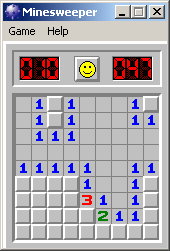
\includegraphics[scale=0.75]{SMT/minesweeper/1.png}
\end{figure}

What we have here, actually? Hidden cells, empty cells (where bombs are not present), and empty cells with numbers, which shows how many bombs are placed nearby.
Here is what we can do: we will try to place a bomb to all possible hidden cells and ask Z3 SMT solver, if it can disprove the very fact that the bomb can be placed there.

\subsubsection{The method}

Take a look at this fragment. "?" mark is for unknown cell, "." is for empty cell, digit is a number of neighbours.

\begin{lstlisting}
_PRE_BEGIN
? ? ?
? 3 .
? 1 .
\end{lstlisting}

So there are 5 unknown cells.
We will try each unknown cell by placing a bomb there.
Let's first pick top/left cell:

\begin{lstlisting}
1 ? ?
? 3 .
? 1 .
\end{lstlisting}

Then we will try to solve the following system of equations (\textit{RrCc} is cell of row r and column c):

\begin{lstlisting}
R1C2+R2C1+R2C2=1                               (because we placed bomb at R1C1)	
R2C1+R2C2+R3C1=1                               (because we have "1" at R3C2)	
R1C1+R1C2+R1C3+R2C1+R2C2+R2C3+R3C1+R3C2+R3C3=3 (because we have "3" at R2C2)	
R1C2+R1C3+R2C2+R2C3+R3C2+R3C3=0                (because we have "." at R2C3)	
R2C2+R2C3+R3C2+R3C3=0                          (because we have "." at R3C3)
\end{lstlisting}

As it turns out, this system of equations is satisfiable, so there could be a bomb at this cell.
But this information is not interesting to us, since we want to find cells we can freely click on.
And we will try another one...

\subsubsection{The code}

\lstinputlisting{SMT/minesweeper/minesweeper_solver.py}

The code is almost self-explanatory.
We need border for the same reason, why Conway's "Game of Life" implementations also has border (to make calculation
function simpler).
Whenever we know that the cell is free of bomb, we put zero there.
Whenever we know number of neighbours, we add a constraint, again, just like in "Game of Life": number of neighbours must be equal to the number we got from the Minesweeper.
Then we place bomb somewhere and check.

Let's run:

\begin{lstlisting}
row=1 col=3, unsat!
row=6 col=2, unsat!
row=6 col=3, unsat!
row=7 col=4, unsat!
row=7 col=9, unsat!
row=8 col=9, unsat!
\end{lstlisting}

These are cells where I can click safely, so I did:

\begin{figure}[H]
\centering
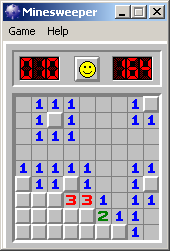
\includegraphics[scale=0.75]{SMT/minesweeper/2.png}
\end{figure}

Now we have more information, so we update input:

\begin{lstlisting}
known=[
"01110001?",
"01?100011",
"011100000",
"000000000",
"111110011",
"?11?1001?",
"???331011",
"?????2110",
"???????10"]
\end{lstlisting}

I run it again:

\begin{lstlisting}
row=7 col=1, unsat!
row=7 col=2, unsat!
row=7 col=3, unsat!
row=8 col=3, unsat!
row=9 col=5, unsat!
row=9 col=6, unsat!
\end{lstlisting}

I click on these cells again:

\begin{figure}[H]
\centering
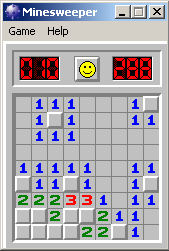
\includegraphics[scale=0.75]{SMT/minesweeper/3.png}
\end{figure}

I update it again:

\begin{lstlisting}
known=[
"01110001?",
"01?100011",
"011100000",
"000000000",
"111110011",
"?11?1001?",
"222331011",
"??2??2110",
"????22?10"]
\end{lstlisting}

\begin{lstlisting}
row=8 col=2, unsat!
row=9 col=4, unsat!
\end{lstlisting}

\begin{figure}[H]
\centering
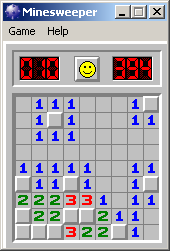
\includegraphics[scale=0.75]{SMT/minesweeper/4.png}
\end{figure}

This is last update:

\begin{lstlisting}
known=[
"01110001?",
"01?100011",
"011100000",
"000000000",
"111110011",
"?11?1001?",
"222331011",
"?22??2110",
"???322?10"]
\end{lstlisting}

... last result:

\begin{lstlisting}
row=9 col=1, unsat!
row=9 col=2, unsat!
\end{lstlisting}

Voila!

\begin{figure}[H]
\centering
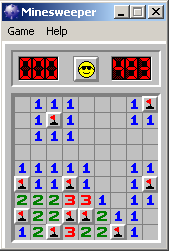
\includegraphics[scale=0.75]{SMT/minesweeper/5.png}
\end{figure}

The source code: \url{https://github.com/dennis714/SAT_SMT_article/blob/master/SMT/minesweeper/minesweeper_solver.py}.

Some discussion on HN: \url{https://news.ycombinator.com/item?id=13797375}.

See also: cracking it using SAT solver: \ref{minesweeper_SAT}.



